%!TEX TS-program = xelatex

% Шаблон документа LaTeX создан в 2018 году
% Алексеем Подчезерцевым
% В качестве исходных использованы шаблоны
% 	Данилом Фёдоровых (danil@fedorovykh.ru) 
%		https://www.writelatex.com/coursera/latex/5.2.2
%	LaTeX-шаблон для русской кандидатской диссертации и её автореферата.
%		https://github.com/AndreyAkinshin/Russian-Phd-LaTeX-Dissertation-Template

\documentclass[a4paper,14pt]{article}


%%% Работа с русским языком
\usepackage[english,russian]{babel}   %% загружает пакет многоязыковой вёрстки
\usepackage{fontspec}      %% подготавливает загрузку шрифтов Open Type, True Type и др.
\defaultfontfeatures{Ligatures={TeX},Renderer=Basic}  %% свойства шрифтов по умолчанию
\setmainfont[Ligatures={TeX,Historic}]{Times New Roman} %% задаёт основной шрифт документа
\setsansfont{Comic Sans MS}                    %% задаёт шрифт без засечек
\setmonofont{Courier New}
\usepackage{indentfirst}
\frenchspacing

\renewcommand{\epsilon}{\ensuremath{\varepsilon}}
\renewcommand{\phi}{\ensuremath{\varphi}}
\renewcommand{\kappa}{\ensuremath{\varkappa}}
\renewcommand{\le}{\ensuremath{\leqslant}}
\renewcommand{\leq}{\ensuremath{\leqslant}}
\renewcommand{\ge}{\ensuremath{\geqslant}}
\renewcommand{\geq}{\ensuremath{\geqslant}}
\renewcommand{\emptyset}{\varnothing}

%%% Дополнительная работа с математикой
\usepackage{amsmath,amsfonts,amssymb,amsthm,mathtools} % AMS
\usepackage{icomma} % "Умная" запятая: $0,2$ --- число, $0, 2$ --- перечисление

%% Номера формул
%\mathtoolsset{showonlyrefs=true} % Показывать номера только у тех формул, на которые есть \eqref{} в тексте.
%\usepackage{leqno} % Нумерация формул слева	

%% Перенос знаков в формулах (по Львовскому)
\newcommand*{\hm}[1]{#1\nobreak\discretionary{}
	{\hbox{$\mathsurround=0pt #1$}}{}}

%%% Работа с картинками
\usepackage{graphicx}  % Для вставки рисунков
\graphicspath{{images/}}  % папки с картинками
\setlength\fboxsep{3pt} % Отступ рамки \fbox{} от рисунка
\setlength\fboxrule{1pt} % Толщина линий рамки \fbox{}
\usepackage{wrapfig} % Обтекание рисунков текстом

%%% Работа с таблицами
\usepackage{array,tabularx,tabulary,booktabs} % Дополнительная работа с таблицами
\usepackage{longtable}  % Длинные таблицы
\usepackage{multirow} % Слияние строк в таблице
\usepackage{float}% http://ctan.org/pkg/float

%%% Программирование
\usepackage{etoolbox} % логические операторы


%%% Страница
\usepackage{extsizes} % Возможность сделать 14-й шрифт
\usepackage{geometry} % Простой способ задавать поля
\geometry{top=20mm}
\geometry{bottom=20mm}
\geometry{left=20mm}
\geometry{right=10mm}
%
%\usepackage{fancyhdr} % Колонтитулы
% 	\pagestyle{fancy}
%\renewcommand{\headrulewidth}{0pt}  % Толщина линейки, отчеркивающей верхний колонтитул
% 	\lfoot{Нижний левый}
% 	\rfoot{Нижний правый}
% 	\rhead{Верхний правый}
% 	\chead{Верхний в центре}
% 	\lhead{Верхний левый}
%	\cfoot{Нижний в центре} % По умолчанию здесь номер страницы

\usepackage{setspace} % Интерлиньяж
\onehalfspacing % Интерлиньяж 1.5
%\doublespacing % Интерлиньяж 2
%\singlespacing % Интерлиньяж 1

\usepackage{lastpage} % Узнать, сколько всего страниц в документе.

\usepackage{soul} % Модификаторы начертания

\usepackage{hyperref}
\usepackage[usenames,dvipsnames,svgnames,table,rgb]{xcolor}
\hypersetup{				% Гиперссылки
	unicode=true,           % русские буквы в раздела PDF
	pdftitle={Автоматизация проектных работ},   % Заголовок
	pdfauthor={Солодянкин А.А.},      % Автор
	pdfsubject={Автоматизация проектных работ},      % Тема
	pdfcreator={Солодянкин А.А.}, % Создатель
	pdfproducer={Солодянкин А.А.}, % Производитель
	pdfkeywords={Автоматизация проектных работ}, % Ключевые слова
	colorlinks=true,       	% false: ссылки в рамках; true: цветные ссылки
	linkcolor=black,          % внутренние ссылки
	citecolor=black,        % на библиографию
	filecolor=magenta,      % на файлы
	urlcolor=black           % на URL
}
\makeatletter 
\def\@biblabel#1{#1. } 
\makeatother
\usepackage{cite} % Работа с библиографией
%\usepackage[superscript]{cite} % Ссылки в верхних индексах
%\usepackage[nocompress]{cite} % 
\usepackage{csquotes} % Еще инструменты для ссылок

\usepackage{multicol} % Несколько колонок

\usepackage{tikz} % Работа с графикой
\usepackage{pgfplots}
\usepackage{pgfplotstable}

% ГОСТ заголовки
\usepackage[font=small]{caption}
%\captionsetup[table]{justification=centering, labelsep = newline} % Таблицы по правобу краю
%\captionsetup[figure]{justification=centering} % Картинки по центру


\newcommand{\tablecaption}[1]{\addtocounter{table}{1}\small \begin{flushright}\tablename \ \thetable\end{flushright}%	
\begin{center}#1\end{center}}

\newcommand{\imref}[1]{рис.~\ref{#1}}

\usepackage{multirow}
\usepackage{spreadtab}
\newcolumntype{K}[1]{@{}>{\centering\arraybackslash}p{#1cm}@{}}


\usepackage{xparse}
\usepackage{fancyvrb}

\RecustomVerbatimCommand{\VerbatimInput}{VerbatimInput}
{
	fontsize=\footnotesize    
}

\newcolumntype{?}[1]{!{\vrule width #1}}

\usepackage{tocloft}
\renewcommand{\cftsecleader}{\cftdotfill{\cftdotsep}}
\begin{document} % конец преамбулы, начало документа
\begin{titlepage}
	\begin{center}
		ПРАВИТЕЛЬСТВО РОССИЙСКОЙ ФЕДЕРАЦИИ \\
 		ФЕДЕРАЛЬНОЕ  ГОСУДАРСТВЕННОЕ АВТОНОМНОЕ \\
		ОБРАЗОВАТЕЛЬНОЕ УЧРЕЖДЕНИЕ ВЫСШЕГО ОБРАЗОВАНИЯ\\
		«НАЦИОНАЛЬНЫЙ ИССЛЕДОВАТЕЛЬСКИЙ УНИВЕРСИТЕТ\\
		«ВЫСШАЯ ШКОЛА ЭКОНОМИКИ»
	\end{center}
	
	\begin{center}
		\textbf{Московский институт электроники и математики}
		
		\textbf{Им. А.Н.Тихонова НИУ ВШЭ}
		
		\vspace{2ex}
		
		\textbf{Департамент компьютерной инженерии}
	\end{center}
	\vspace{1ex}	
	
	\vspace{1ex}
	\begin{center}
		\textbf{Практическая работа №7 \\
			<<Математические модели для решения задач размещения на печатной плате>> \\
			по курсу <<Автоматизация проектных работ>>\\
	}
	\end{center}	

	\vspace{2ex}
	\vfill
	
	\vspace{2ex}
	
	\begin{flushright}
		\textbf{Выполнил:}
		
		\vspace{2ex}
		
		Студент группы БИВ174
		
		\vspace{2ex}
		
		Солодянкин Андрей Александрович
		
		\vspace{2ex}
		
		\textbf{Проверил:}
		
		\vspace{2ex}
		
		Новиков Константин Викторович
	\end{flushright}

	\vspace{5ex}
	\begin{center}
		Москва \the\year \, г.
	\end{center}
	
\end{titlepage}
\addtocounter{page}{1}
\tableofcontents
\pagebreak

\section{Задание}

Изучение методов математичекого моделирования электрических схем в статическом режиме.
Изучение способов обеспечения ститического режима работы схем методами математического моделирования.

\section{Краткие теоретические сведения}

Транзисторные сглаживающие фильтры.
Уменьшить массогабаритные показатели можно, используя транзисторные СФ, вместо громоздких LC-фильтров. 
Правда выигрыш транзисторных фильтров компенсируется меньшим КПД.
Рассмотрим типичные схемы транзисторных фильтров.
На рис.~\ref{fig:method1} представлена схема наиболее простого транзисторного фильтра.

\begin{figure}[H]
	\centering
	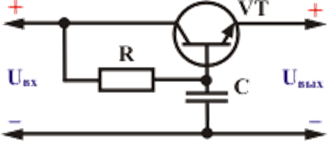
\includegraphics[width=0.5\linewidth]{image/method_1}
	\caption{Простейший транзисторный фильтр}
	\label{fig:method1}
\end{figure}

На коллектор транзистора VT поступает напряжение с выпрямителя с большой амплитудой пульсаций. 
Цепь базы питается через интегрирующую цепь RC. 
Эта цепочка сглаживает пульсации на базе транзистора.
В принципе, эту цепь можно представить, как RC-фильтр.
Чем больше постоянная времени τ = RC, тем меньше пульсации напряжения на базе транзистора.
Ну а поскольку транзистор включен по схеме эмиттерного повторителя, то на выходе напряжение будет повторять напряжение на базе, т. е. пульсации будут столь же малыми, как и на базе.
Емкость конденсатора С может быть в несколько раз меньше (примерно в h21э раз), чем в LC-фильтре, поскольку базовый ток намного меньше выходного тока фильтра, т. е. коллекторного тока транзистора.
Основное достоинство схемы - простота.
А вот недостатков...
Во-первых, противоречивые требования к сопротивлению резистора R - для уменьшения пульсаций следует увеличивать сопротивление, для повышения КПД - уменьшать.
Во-вторых, сильная зависимость параметров от температуры, тока нагрузки, коэффициента передачи тока базы транзистора (h21э).
Обычно резистор подбирают экспериментально.
Несколько иная схема, приведенная на рис.~\ref{fig:method2}.
В такой схеме цепь базы транзистора запитывается от отдельного источника с напряжением, больше входного.
Схема обладает меньшими пульсациями.

\begin{figure}[H]
	\centering
	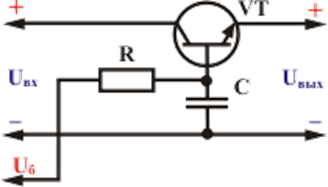
\includegraphics[width=0.5\linewidth]{image/method_2}
	\caption{Еще одна схема транзисторного СФ}
	\label{fig:method2}
\end{figure}

Поскольку база питается от отдельного источника, сопротивление резистора можно увеличить и, следовательно, уменьшить пульсации выходного напряжения.
Мощность, выделяемая на резисторе R мала, так как ток базы мал.
Тем не менее, этой схеме присущи те же недостатки, что и предыдущей.
Кроме того, в таком фильтре транзистор может войти в насыщение и все пульсации со входа фильтра без ограничений будут передаваться на выход.
В этот режим транзистор войдет, когда напряжение на базе превысит напряжение на коллекторе.
Ниже приведена схема транзисторного СФ, лишенная вышеуказанных недостатков.

\begin{figure}[H]
	\centering
	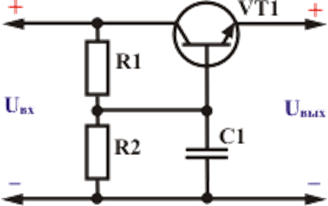
\includegraphics[width=0.5\linewidth]{image/method_3}
	\caption{Фильтр с делителем напряжения}
	\label{fig:method3}
\end{figure}

\section{Выполнение работы}

На рис. \ref{fig:shem} приведена электрическая схема фильтра.

\begin{figure}[H]
	\centering
	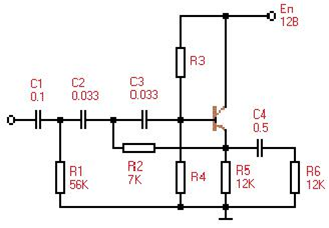
\includegraphics[width=0.7\linewidth]{image/shem}
	\caption{Электрическая схема фильтра}
	\label{fig:shem}
\end{figure}


На рис.~\ref{fig:work2} показаны результаты моделирования статического режима СФ.
При $R_3$ = 3кОм и $R_4$ = 3.7кОм на эмиттере транзистора напряжение равно половине напряжения питания, 6В.

\begin{figure}[H]
	\centering
	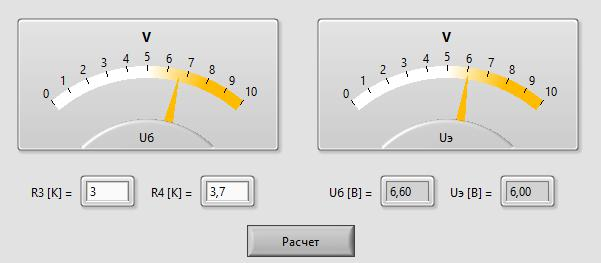
\includegraphics[width=0.7\linewidth]{image/work2}
	\caption{Результат моделирования}
	\label{fig:work2}
\end{figure}


\section{Выводы по работе}

В ходе выполнения лабораторной работы были изучены методы математического моделирования электрических схем в статическом режиме, способы обеспечения статического режима работы схем методами математического моделирования, был обеспечен статический режим работы транзисторного фильтра таким образом, что напряжение на эмиттере транзистора стало равным половине напряжения питания – 6В.
\section{Контрольные вопросы}

\begin{enumerate}
	\item Метод Ньютона-Рафсона для расчета статического режима электрических схем.
	
	Пусть на отрезке $[a,b]$ существует единственный корень уравнения: $f(x^*)=0$, 
	а $f'(x)$ существует, непрерывна и отлична от нуля на $[a,b]$. Перепишем уравнение следующим образом: $f(x^k+(x^*-x^k))=0$
	и применим к этому выражению формула Лагранжа:
	$f(x^k)+f'(\bar{x})(x^*-x^k)=0, \;\bar{x} \in [a,b]$
	Заменим $ \bar x$ на $x^k$, а $x^*$ - на $x^{k+1}$ и получим формулу итерационного процесса:
    $f(x^k)+f'(x^k)(x^{k+1}-x^k)=0.$
	Выразим отсюда $x^{k+1}$:
	
	$x^{k+1}=x^k-\frac{f(x^k)}{f'(x^k)}$
	
	\item Условия сходимости метода Ньютона-Рафсона.

	Метод касательных является частным случаем метода простых итераций $x^{k+1} = g(x^k), k = 0,1,...$
	
	Для которого $g(x) = x - \frac{f(x)}{f'(x)}$
	
	Метод простых итераций сходится тогда и только тогда, когда $|g'(x)|\leq q<1$,
	
	Подставим в последнее условие выражение для g(x) и получим условие сходимости метода касательных:
	
	$\dfrac{\left|f'(x)f''(x) \right|}{(f'(x))^2} \leq q < 1 $
	
%	$ lim | V - V^*| = 0$
	
	\item Метод продолжения решения по параметру
		
	Введем систему нелинейных алгебраических уравнений: 
	
	$$I'(V,t) = 0$$
	
	где t – параметр, изменяющийся от 0 до 1, такой, что при t=0 
	
	$$I'(V,0) =0$$
	
	имеет известное решение $V^0$, а при $t=1 I'(V,1)=0$, соответствующее решению системы уравнений.
	
	При этом основное требование заключается в том, чтобы функция $I'(V,t)$ была непрерывной при изменении t от 0 до 1.
	Тогда изменяя параметр $t$ от 0 до 1 и решая для каждого $t$ систему уравнений методом Ньютона-Рафсона можно найти последовательность $V^0, V^1,...,V^*$и получить требуемое решение.
	
	\item Объясните почему напряжение на эмиттере транзистора должно быть равно половине напряжения питания.
	
	Для получения максимального значения амплитуды выходного неискаженного сигнала рекомендуется задавать напряжение коллектор-эмиттер в точке покоя равным половине напряжения питания.
\end{enumerate}

\end{document} % конец документа